\documentclass[margin=0px]{article}

\usepackage{listings}
\usepackage[utf8]{inputenc}
\usepackage{graphicx}
\usepackage{float}
\usepackage[a4paper, margin=0.7in]{geometry}
\usepackage{amsthm}
\usepackage{amssymb}
\usepackage{fancyhdr}
\usepackage{setspace}

\onehalfspacing

\makeatletter
\renewcommand\paragraph{%
	\@startsection{paragraph}{4}{0mm}%
	{-\baselineskip}%
	{.5\baselineskip}%
	{\normalfont\normalsize\bfseries}}
\makeatother

\renewcommand{\figurename}{ábra}

\newenvironment{tetel}[1]{\paragraph{#1 \\}}{}

\pagestyle{fancy}
\lhead{\it{PTI BSc Záróvizsga tételek}}
\rhead{13. Számításelmélet}

\title{\textbf{{\Large ELTE IK - Programtervező Informatikus BSc} \vspace{0.2cm} \\ {\huge Záróvizsga tételek}} \vspace{0.3cm} \\ 13. Számításelmélet}
\author{}
\date{}

\begin{document}
\maketitle

\begin{tetel}{Számításelmélet}
    A Turing gép és a Church-Turing tézis. Turing gépek variánsok: többszalagos, nemdeterminisztikus, számoló, offline. Rekurzív és rekurzívan felsorolható nyelvek. Eldönthetetlen problémák. Idő- és tárbonyolultsági osztályok: P, NP, PSPACE. NP-teljes problémák.
\end{tetel}

\section{Kiszámíthatóság}

\subsubsection{Algoritmusmodellek}

\begin{itemize}
    \item	\textbf{Gödel}: rekurzív függvények (primitív rekurzív függvények 1931-ben, majd általánosabb 1934-ben)

    \item	\textbf{Church}: $\lambda$-kalkulus, $\lambda$-definiálható függvények: ekvivalensek a rekurzív függvényekkel (bizonyított)

    \item	\textbf{Turing}: Turing-gép (1936), a $\lambda$-definiálható és a Turing-géppel kiszámítható függvények megegyeznek (bizonyított)

\end{itemize}

\noindent \textbf{Church-Turing tézis}: A kiszámíthatóság különböző matematikai modelljei mind az effektíven
kiszámítható függvények osztályát definiálják.

\subsubsection{Fogalmak}

Kiszámítási problémának nevezünk egy olyan, a matematika nyelvén megfogalmazott
kérdést, amire egy algoritmussal szeretnénk megadni a választ. A
gyakorlati élet szinte minden problémájához rendelhető, megfelelő absztrakciót
használva, egy kiszámítási probléma.\\

\noindent Egy problémát a hozzá tartozó konkrét bementettel együtt a probléma egy
példányának nevezzük.\\

Speciális kiszámítási probléma az eldöntési probléma. Ilyenkor a problémával
kapcsolatos kérdés egy eldöntendő kérdés, tehát a probléma egy példányára a
válasz "igen" vagy "nem" lesz.\\

Egy kiszámítási probléma reprezentálható egy $f : A \to B$ függvénnyel. Az $A$
halmaz tartalmazza a probléma egyes bemeneteit, jellemzően egy megfelelő ábécé
feletti szóban elkódolva, míg a $B$ halmaz tartalmazza a bemenetekre adott
válaszokat, szintén valamely alkalmas ábécé feletti szóban elkódolva. Értelemszerűen,
ha eldöntési problémáról van szó, akkor az $f$ értékkészlete, vagyis a $B$
egy két elemű halmaz: $\left\{igen, nem\right\}$, $\left\{1, 0\right\}$, stb.\\

\noindent \textbf{Kiszámítható függvény}: Egy $f : A \to B$ függvényt \textit{kiszámíthatónak}
nevezünk, ha minden $x \in A$ elemre az $f(x) \in B$ függvényérték kiszámítható valamilyen
algoritmikus modellel.\\

\noindent \textbf{Megoldható, eldönthető probléma}: Egy kiszámítási probléma \textit{megoldható}
(eldöntési probléma esetén azt mondjuk, hogy \textit{eldönthető}), ha az általa meghatározott
függvény kiszámítható.\\

\noindent \textbf{Algoritmusok időigénye}: Legyenek $f,g: \mathbb{N} \to \mathbb{N}$ függvények, ahol
$\mathbb{N}$ a természetes számok halmaza. Azt mondjuk, hogy $f$ legfeljebb olyan gyorsan nő, mint $g$
(jelölése: $f(n) = \mathcal{O}(g(n))$), ha $\exists c>0$ és $n_{0} \in \mathbb{N}$, hogy
$f(n) \leq c * g(n) \ \forall n \geq n_{0}$. Az $f(n) = \Omega(g(n))$ jelöli azt, hogy $g(n) = \mathcal{O}(f(n))$
teljesül és $f(n) = \Theta(g(n))$ jelöli azt, hogy  $f(n) = \mathcal{O}(g(n))$ és $f(n) = \Omega(g(n))$ is teljesül.\\

\noindent \textbf{Példa}: $3n^{3} + 5n^{2} + 6 = \mathcal{O}(n^{3})$, $n^{k} = \mathcal{O}(2^{n}) \ \forall k \geq 0$, stb.\\

\noindent \textbf{Tétel}: Minden polinomiális függvény lassabban nő, mint bármely exponenciális függvény,
azaz minden $p(n)$ polinomhoz és $c>0$-hoz $\exists n_{0}$ egész szám, hogy $\forall n \geq n_{0}$ esetén $p(n) \leq 2^{cn}$\\

\noindent \textbf{Kiszámítási probléma megfeleltetése eldöntési problémának}: Tekintsünk egy $P$ kiszámítási problémát
és legyen $f: A \to B$ a $P$ által meghatározott függvény. Ekkor megadható $P$-hez egy $P'$ eldöntési probléma úgy, hogy
$P'$ pontosan akkor eldönthető, ha $P$ kiszámítható. Állítsuk párba ugyanis minden $a \in A$ elemre az $a$ és $f(a)$ elemeket,
és kódoljuk el az így kapott párokat egy-egy szóban. Ezek után legyen $P'$ az így kapott szavakból képzett formális nyelv.
Nyilvánvaló, hogy ha minden $a \in A$ és $b \in B$ elemre az $(a,b) \in P'$ tartalmazás eldönthető (azaz $P'$ eldönthető), akkor
$P$ kiszámítható és fordítva.
E megfeleltetés miatt a továbbiakban jellemzően eldöntési problémákkal foglalkozunk.

\section{Turing-gépek}

Hasonlóan a véges automatához vagy a veremautomatához, a Turing-gép is
egy véges sok állapottal rendelkező eszköz. A Turing-gép egy két irányban
végtelen szalagon dolgozik. A szalag cellákra van osztva, tulajdonképpen ez
a gép (korlátlan) memóriája. Kezdetben a szalagon csak a bemenő szó van,
minden cellán egy betű. A szalag többi cellája egy úgynevezett blank vagy
szóköz ($\sqcup$) szimbólumokkal van feltöltve. Kezdetben a gép úgynevezett író-olvasó
feje a bemenő szó első betűjén áll és a gép a kezdőállapotában van.
A gép az író-olvasó fejet tetszőlegesen képes mozgatni a szalagon. Képes továbbá
a fej pozíciójában a szalag tartalmát kiolvasni és átírni. A gépnek van két
kitüntetett állapota, a $q_{i}$ és a $q_{n}$ állapotok. Ha ezekbe az állapotokba kerül,
akkor rendre elfogadja illetve elutasítja a bemenő szót.
Formálisan a Turing-gépet a következő módon definiáljuk.\\

\noindent \textbf{A Turing-gép formális definíciója}: A Turing-gép egy olyan
$M = (Q, \Sigma, \Gamma, \delta, q_{0}, q_{i}, q_{n})$ rendszer, ahol:

\begin{itemize}

    \item	$Q$ az állapotok véges, nem üres halmaza,

    \item	$q_{0}, q_{i}, q_{n} \in Q$, $q_{0}$ a kezdőállapot, $q_{i}$ az elfogadó állapot,
          $q_{n}$ pedig az elutasító állapot,

    \item	$\Sigma$ és $\Gamma$ ábécék, a bemenő jelek és a szalagszimbólumok ábécéje úgy, hogy
          $\Sigma \subseteq \Gamma$ és $\Gamma - \Sigma$ tartalmaz egy speciális $\sqcup$ szimbólumot,

    \item	$\delta : (Q - \left\{q_{i},q_{n}\right\}) \times \Gamma \to Q \times \Gamma \times \left\{L, R, S\right\}$
          az átmenetfüggvény.

\end{itemize}

Úgy mint a veremautomaták esetében, egy $M$ Turing-gép működésének fázisait	is konfigurációkkal írhatjuk le.\\

\noindent \textbf{Turing-gép konfigurációja}: Az $M$ Turing-gép konfigurációja egy olyan $uqv$ szó, ahol
$q \in Q$ és $u, v \in \Gamma^{*}$, $v \not = \varepsilon$. Ez a konfiguráció az $M$ azon állapotát tükrözi
amikor a szalag tartalma $uv$ ($uv$ előtt és után a szalagon már csak $\sqcup$ van), a gép a $q$ állapotban van,
és az író-olvasó fej a $v$ első betűjére mutat. $M$ összes konfigurációjának halmazát $\mathcal{C}_{M}$-el jelöljük.\\

\noindent \textbf{Turing-gép kezdőkonfigurációja}: $M$ kezdőkonfigurációja egy olyan $q_{0}u\sqcup$ szó, ahol
$u$ csak $\Sigma$-beli betűket tartalmaz.\\

\noindent \textbf{Turing-gép konfigurációátmenete}: $M$ konfigurációátmenete egy olyan
$\vdash \subseteq \mathcal{C}_{M} \times \mathcal{C}_{M}$ reláció, amit a következőképpen definiálunk.
Legyen $uqav$ egy konfiguráció, ahol $a \in \Gamma$ és $u, v \in \Gamma^{*}$. A következő három esetet
különböztetjük meg:

\begin{enumerate}

    \item	Ha $\delta(q,a) = (r, b, S)$, akkor $uqav \vdash urbv$.

    \item	Ha $\delta(q,a) = (r, b, R)$, akkor $uqav \vdash ubrv'$, ahol $v' = v$, ha $v \not = \varepsilon$, különben
          $v' = \sqcup$.

    \item	Ha $\delta(q,a) = (r, b, L)$, akkor $uqav \vdash u'rcbv$, ahol $u'c = u$ valamely $u' \in \Gamma^{*}$-ra
          és $c \in \Gamma$-ra, ha $u \not = \varepsilon$, egyébként pedig $u' = \varepsilon$, $c = \sqcup$.

\end{enumerate}

Azt mondjuk, hogy $M$ véges sok lépésben eljut a $C$ konfigurációból a  $C'$ konfigurációba (jele $C \vdash^{*} C'$),
ha létezik olyan $n \geq 0$ és $C_{1}, ... C_{n}$ konfigurációsorozat, hogy $C_{1} = C$, $C_{n} = C'$ és minden
$1 \leq i < n$-re $C_{i} \vdash C_{i+1}$.

Ha $q \in \left\{q_{i}, q_{n}\right\}$, akkor azt mondjuk, hogy az $uqv$ konfiguráció egy megállási
konfiguráció. Továbbá, $q = q_{i}$ esetében elfogadó, míg $q = q_{n}$ esetében elutasító
konfigurációról beszélünk.\\

\noindent \textbf{Turing-gép által felismert nyelv}: Az $M$ Turing-gép által felismert nyelv (jelölése $L(M)$)
azoknak az $u \in \Sigma^{*}$ szavaknak a halmaza, melyekre igaz, hogy $q_{0}u\sqcup \vdash^{*} xq_{i}y$
valamely $x,y \in \Gamma^{*}$, $y \not = \varepsilon$ szavakra.

\begin{figure}[H]
    \centering
    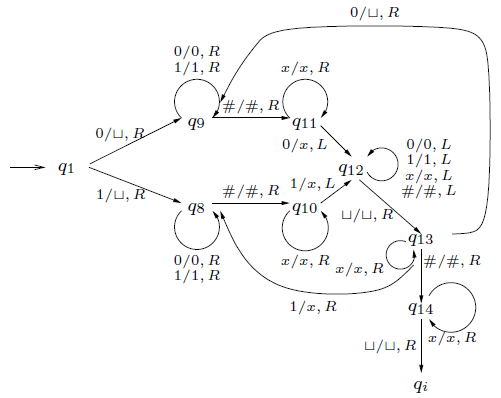
\includegraphics[width=0.6\linewidth]{img/turinggep_pelda}
    \caption{Egy, az $L = \left\{u\#u \ | \ u \in \left\{0,1\right\}^{+}\right\}$ felismerő Turing-gép.}
    \label{fig:turinggep_pelda}
\end{figure}

\noindent \textbf{Turing-gépek ekvivalenciája}: Két Turing-gépet ekvivalensnek nevezünk, ha ugyanazt a nyelvet ismerik fel.\\

\noindent \textbf{Turing-felismerhető nyelv, rekurzívan felismerhető nyelvek osztálya}:
Egy $L \subseteq \Sigma^{*}$ nyelv Turing-felismerhető, ha	$L = L(M)$ valamely $M$ Turing-gépre.
A Turing-felismerhető nyelveket szokás \textit{rekurzívan felsorolhatónak} is nevezni.
A rekurzívan felsorolható nyelvek osztályát $RE$-vel jelöljük.\\

\noindent \textbf{Turing-eldönthető nyelv, rekurzív nyelvek osztálya}:
Egy $L \subseteq \Sigma^{*}$ nyelv Turing-eldönthető, ha létezik olyan Turing-gép,
amely minden bemeneten megállási konfigurációba jut és felismeri $L$-et.
A Turing-felismerhető nyelveket szokás \textit{rekurzívnak} is nevezni.
A rekurzív nyelvek osztályát $R$-rel jelöljük.\\

\noindent \textbf{Turing-gép futási ideje, időigénye}:
Tekintsünk egy $M = (Q, \Sigma, \Gamma, \delta, q_{0}, q_{i}, q_{n})$ Turing-gépet és annak egy
$u \in \Sigma^{*}$ bemenő szavát. Azt mondjuk, hogy $M$ futási ideje (időigénye) az $u$ szón $n$ ($n \geq 0$),
ha $M$ a $q_{0}u\sqcup$ kezdőkonfigurációból $n$ lépésben el tud jutni egy megállási konfigurációba. Ha nincs ilyen
szám, akkor $M$ futási ideje az $u$ szón végtelen.

Legyen $f : \mathbb{N} \to \mathbb{N}$ egy függvény. Azt mondjuk, hogy $M$ időigénye $f(n)$ (vagy azt, hogy $M$
egy $f(n)$ időkorlátos gép), ha minden $u \in \Sigma^{*}$ input szóra $M$ időigénye az $u$ szón legfeljebb $f(l(u))$.

\subsubsection{Többszalagos Turing-gépek}

A többszalagos Turing-gépek, értelemszerűen, egynél több szalaggal rendelkeznek.
Mindegyik szalaghoz tartozik egy-egy író-olvasó fej, melyek egymástól
függetlenül képesek mozogni a szalagon.\\

\noindent \textbf{Többszalagos Turing-gép definíciója}: Legyen $k > 1$. Egy $k$-szalagos Turing-gép egy olyan
$M = (Q, \Sigma, \Gamma, \delta, q_{0}, q_{i}, q_{n})$ rendszer, ahol a komponensek a $\delta$ kivételével
megegyeznek az egyszalagos Turing-gép komponenseivel, $\delta$ pedig a következőképpen adódik.
$\delta : (Q - \left\{q_{i},q_{n}\right\}) \times \Gamma^{k} \to Q \times \Gamma^{k} \times \left\{L, R, S\right\}^{k}$.
Legyenek $q, p \in Q$, $a_{1}, a_{2}, ... , a_{k}, b_{1}, b_{2}, ..., b_{k} \in \Gamma$ és
$D_{1}, D_{2}, ..., D_{k} \in \left\{L, R, S\right\}$. Ha $\delta(q,a_{1}, a_{2}, ... , a_{k}) = (p,b_{1}, b_{2}, ..., b_{k}, D_{1}, D_{2}, ..., D_{k})$, akkor a gép akkor a gép a $q$ állapotból, ha a szalagjain rendre az
$a_{1}, a_{2}, ... , a_{k}$ betűket olvassa, át tud menni a $p$ állapotba, miközben az
$a_{1}, a_{2}, ... , a_{k}$ betűket átírja a $b_{1}, b_{2}, ... , b_{k}$ betűkre és a szalagokon a fejeket
$D_{1}, D_{2}, ... , D_{k}$ irányokba mozgatja.

A többszalagos Turing-gép konfigurációja, a konfigurációátmenet valamint a
felismert illetve eldöntött nyelv definíciója az egyszalagos eset értelemszerű általánosítása.
A többszalagos Turing-gép időigényét is az egyszalagoshoz hasonlóan	definiáljuk.\\

\noindent \textbf{Többszalagos és egyszalagos gépek ekvivalenciája}: Minden $k$-szalagos, $f(n)$ időkorlátos Turing-géphez
van vele ekvivalens $\mathcal{O}(n*f(n))$ időkorlátos egyszalagos Turing-gép.

\subsubsection{Nemdeterminisztikus Turing-gépek}

Egy $M$ nemdeterminisztikus Turing-gép állapotfüggvénye
$\delta : (Q - \left\{q_{i},q_{n}\right\}) \times \mathcal{P}(\Gamma \to Q \times \Gamma \times \left\{L, R\right\})$
alakú. Tehát $M$ minden konfigurációjából néhány (esetleg nulla) különböző konfigurációba mehet át.
Ily módon $M$ számítási sorozatai egy $u$ szón egy fával reprezentálhatók. A fa csúcsa $M$ kezdőkonfigurációja,
a szögpontjai pedig	$M$ konfigurációi. A fa minden levele megfelel $M$ egy számítási sorozatának az
$u$-n. $M$ akkor fogadja el $u$-t, ha a fa valamelyik levele elfogadó konfiguráció.
Nevezzük ezt a most leírt fát az $M$ nemdeterminisztikus számítási fájának az
$u$-n. Az $M$ által felismert nyelv a determinisztikus esethez hasonlóan definiálható,
a gép által eldöntött nyelv pedig a következőképpen.\\

\noindent \textbf{Nemdeterminisztikus Turing-gép által eldöntött nyelv}: Azt mondjuk, hogy egy nemdeterminisztikus
$M$ Turing-gép eldönt egy $L \subseteq \Gamma^{*}$ nyelvet, ha felismeri, és minden $u \in \Sigma{*}$ szóra
$M$ számítási sorozatai végesek és elfogadási vagy elutasítási konfigurációba vezetnek.\\

\noindent \textbf{Nemdeterminisztikus Turing-gép időigénye}: Legyen $f : \mathbb{N} \to \mathbb{N}$ függvény, $M$
egy nemdeterminisztikus Turing-gép. Az $M$ időigénye $f(n)$, ha egy $n$ hosszú $u$ bemeneten nincsenek $M$-nek
$f(n)$-nél hosszabb számítási sorozatai, azaz az $M$ számítási fája az $u$-n legfeljebb $f(n)$ magas.\\

\noindent \textbf{Determinisztikus és nemdeterminisztikus Turing-gépek ekvivalenciája}:
Minden $M$ nemdeterminisztikus Turing-géphez megadható egy ekvivalens $M'$ determinisztikus Turing-gép.
Továbbá, ha $M$ $f(n)$ időigényű valamely $f : \mathbb{N} \to \mathbb{N}$ függvényre, akkor
$M'$ $2^{\mathcal{O}(f(n))}$ időigényű.


\section{Eldönthetetlen problémák}

Ebben a fejezetben megmutatjuk, hogy bár a Turing-gép a lehető legáltalánosabb
algoritmus modell, mégis vannak olyan problémák, melyek nem számíthatók ki Turing-géppel.\\

\noindent \textbf{Emlékeztető}: A rekurzívan felsorolható (Turing-felismerhető) nyelvek osztályát $RE$-vel,
a rekurzív (Turing-eldönthető) nyelvek osztályát $R$-rel jelöljük.\\

Világos, hogy $R \subseteq RE $. A célunk az, hogy megmutassuk: az $R$ valódi részhalmaza az $RE$-nek,
azaz van olyan nyelv (probléma) ami	Turing-felismerhető, de nem eldönthető.

Csak olyan Turing-gépeket fogunk vizsgálni, melyek bemenő ábécéje a $\left\{0, 1\right\}$ halmaz.
Ez nem jelenti az általánosság megszorítását, hiszen ha	találunk egy olyan $\left\{0, 1\right\}$ feletti nyelvet,
melyet nem lehet eldönteni ilyen Turing-géppel, akkor ezt a nyelvet egyáltalán nem lehet eldönteni.\\

\subsubsection{Turing-gépek kódolása}

A $\left\{0, 1\right\}$ feletti szavak felsorolhatóak (vagyis megszámlálhatóak). Valóban, tekintsük azt a felsorolást,
amelyben a szavak a	hosszuk szerint követik egymást, és két egyforma hosszú szó közül pedig az van
előbb, amelyik az alfabetikus rendezés szerint megelőzi a másikat. Ily módon
a $\left\{0, 1\right\}^{*}$ halmaz elemeinek egy felsorolása a következőképpen alakul: $w_{1} = \varepsilon$,
$w_{2} = 0$, $w_{3} = 1$, $w_{4} = 00$, $w_{5} = 01$ és így tovább. Ebben a fejezetben tehát a
$w_{i}$ szóval a $\left\{0, 1\right\}^{*}$ $i$. elemét jelöljük.

Legyen továbbá $M$ egy $\left\{0, 1\right\}$ inputábécé feletti Turing-gép. Van olyan $k > 0$ szám, hogy
$Q$-t felírhatjuk $Q = \left\{p_{1}, ... p_{k}\right\}$ alakban, ahol $p_{1} = q_{0}$, $p_{k-1} = q_{i}$, $p_{k} = q_{n}$.
Továbbá, van olyan $m > 0$ szám, hogy $\Gamma$-t felírhatjuk $\Gamma = \left\{X_{1}, ... X_{m}\right\}$ alakban,
ahol $X_{1} = 0$, $X_{2} = 1$, $X_{3} = \sqcup$, és $X_{4}, ... X_{m}$ az $M$ további szalagszimbólumai.
Nevezzük végül az $L, R, S$ szimbólumokat (amelyek irányokat jelölnek) rendre $D_{1}$, $D_{2}$ és $D_{3}$-nak.
Ezek után $M$ egy $\delta(p_{i},X_{j}) = (p_{r}, X_{s}, D_{t})$ ($0 \leq i,r \leq k$, $1 \leq j,s \leq m$ és $1 \leq t \leq 3$)
átmenete elkódolható a $0^{i}10^{j}10^{r}10^{s}10^{t}$ szóval. Mivel minden $0$-s blokk hossza legalább $1$, az átmenetet
kódoló szóban nem szerepel az $11$ részszó. Tehát az M összes átmenetét kódoló szavakat összefűzhetjük egy olyan szóvá,
melyben az átmeneteket az $11$ részszó választja el egymástól. Az így kapott szó pedig magát $M$-et kódolja.\\

A továbbiakban $M_{i}$-vel jelöljük azt a Turing-gépet, amelyet a $w_{i}$ szó kódol ($i \geq 1$). Amennyiben
$w_{i}$ nem a fent leírt kódolása egy Turing-gépnek, akkor tekintsük $M_{i}$-t olyannak, ami minden input esetén
azonnal a $q_{n}$ állapotba megy, azaz $L(M_{i}) = \emptyset$.\\

A későbbiekben szükségünk lesz arra, hogy elkódoljunk egy $(M, w)$ Turing-gép és bemenet
párost egy $\left\{0, 1\right\}$ feletti szóban. Mivel a Turing-gépek kódolása nem tartalmazhat
$111$-et, ezért $(M, w)$ kódja a következő: $M$ kódja után írunk $111$-et, majd utána $w$-t.

\subsubsection{Egy nem rekurzívan felsorolható nyelv}

\noindent \textbf{Az $L_{\acute{a}tl\acute{o}}$ nyelv}: Az $L_{\acute{a}tl\acute{o}}$ nyelv azon $\left\{0, 1\right\}$
feletti Turing-gépek bináris kódjait tartalmazza, melyek nem fogadják el önmaguk kódját, mint bemenő szót, azaz
$L_{\acute{a}tl\acute{o}} = \left\{w_{i} \ | \ i \geq 1, w_{i} \notin L(M_{i}) \right\}$\\

\noindent \textbf{Tétel}: $L_{\acute{a}tl\acute{o}} \notin RE$.

\subsubsection{Egy rekurzívan felsorolható, de nem eldönthető nyelv}

\noindent \textbf{Az $L_{u}$ nyelv}: Tekintsük azon $(M, w)$ párok halmazát (egy megfelelő bináris szóban elkódolva),
ahol $M$ egy $\left\{0, 1\right\}$	bemenő ábécé feletti Turing-gép, $w$ pedig egy $\left\{0, 1\right\}$ feletti
szó úgy, hogy $w \in L(M)$, azaz $M$ elfogadja $w$-t. Ezt a nyelvet jelöljük $L_{u}$-val.
$L_{u} = \left\{\langle w_{i},w_{j} \rangle \ | \ i, j \geq 1, w_{j} \in L(M_{i}) \right\}$\\

\noindent \textbf{Tétel}: $L_{u} \in RE$.\\

\noindent \textbf{Tétel}: $L_{u} \notin R$.

\subsubsection{További tételek}

\begin{enumerate}
    \item	Legyen $L$ egy nyelv. Ha $L, \bar{L} \in RE$, akkor $L \in R$. Következmény: a rekurzívan felsorolható
          nyelvek nem zártak a komplementerképzésre.

    \item	Ha $L \in R$, akkor $\bar{L} \in R$, azaz a rekurzív nyelvek zártak a komplementerképzésre.
\end{enumerate}

\subsubsection{További eldönthetetlen problémák}

\noindent \textbf{Kiszámítható függvény}: Legyen $\Sigma$ és $\Delta$ két ábécé és $f$ $\Sigma^{*}$ból
$\Delta^{*}$-ba képző függvény. Azt mondjuk, hogy $f$ kiszámítható, ha van olyan $M$ Turing-gép, hogy
$M$-et egy $w \in \Sigma^{*}$ szóval a bemenetén elindítva, $M$ úgy áll meg, hogy a szalagján a
$f(w) \in \Delta^{*}$ szó van.\\

\noindent \textbf{Eldöntési problémák visszavezetése}: Legyen $L_{1} \subseteq \Sigma^{*}$ és $L_{2} \subseteq \Delta^{*}$
két eldöntési probléma. $L_{1}$ visszavezethető $L_{2}$-re ($L_{1} \leq L_{2}$), ha van olyan
$f : \Sigma^{*} \to \Delta^{*}$ kiszámítható függvény, hogy minden $w \in \Sigma^{*}$ szóra
$w \in L_{1}$ pontosan akkor teljesül, ha $f(w) \in L_{2}$ is teljesül.\\

\noindent \textbf{Tétel}: Legyen $L_{1} \subseteq \Sigma^{*}$ és $L_{2} \subseteq \Delta^{*}$
két eldöntési probléma és tegyük fel, hogy $L_{1}$ visszavezethető $L_{2}$-re. Ekkor igazak a következő állítások:

\begin{enumerate}
    \item	Ha $L_{1}$ eldönthetetlen, akkor $L_{2}$ is.

    \item	Ha $L_{1} \notin RE$ , akkor $L_{2} \notin RE$.
\end{enumerate}

\noindent \textbf{A megállási probléma}: Legyen $L_{h} = \left\{\langle M, w \rangle \ |\ M \ meg\acute{a}ll \ a \ w \ bemeneten \right\}$,
azaz $L_{h}$ azon $\langle M, w \rangle$ Turing-gép és bemenet párosokat tartalmazza elkódolva, melyekre $M$ megáll a $w$ bemeneten.
$L_{h}$ eldönthetetlen ($L_{u}$ visszavezethető $L_{h}$-ra), viszont $L_{h} \in RE$.\\

\noindent \textbf{Az $L_{\ddot{u}res}$ probléma}: Legyen $L_{\ddot{u}res} = \left\{\langle M \rangle \ |\ L(M) = \emptyset \right\}$.
$L_{\ddot{u}res}$ eldönthetetlen ($L_{u}$ visszavezethető $L_{\ddot{u}res}$-re), valamint $L_{\ddot{u}res} \notin RE$.\\

\noindent \textbf{Rekurzívan felsorolható nyelvek (nem triviális) tulajdonsága}: Ha $\mathcal{P}$ a rekurzívan felsorolható
nyelvek egy halmaza, akkor $\mathcal{P}$ a rekurzívan felsorolható nyelvek egy tulajdonsága. Ha $\mathcal{P} \not = \emptyset$ és
$\mathcal{P} \not = RE$, akkor $\mathcal{P}$ nem triviális tulajdonsága a rekurzívan felsorolható nyelveknek.\\

\noindent \textbf{Rice tétele}:
Adott $\mathcal{P}$ tulajdonságra jelöljük $L_{\mathcal{P}}$-vel azon Turing-gépek kódjainak halmazát, amelyek
$\mathcal{P}$-beli nyelvet ismernek fel. Ha $\mathcal{P}$ a rekurzívan felsorolható nyelvek egy nem triviális tulajdonsága, akkor
$L_{\mathcal{P}}$ eldönthetetlen.\\

\noindent \textbf{Post Megfelelkezési Probléma (röviden PMP)}: A PMP problémát a következőképpen definiáljuk. Legyen
$\Sigma$ egy legalább két betűt tartalmazó ábécé és legyen $D = \left\{[\frac{u_{1}}{v_{1}}], ..., [\frac{u_{n}}{v_{n}}]\right\}$
egy dominóhalmaz, melyben $n \geq 1$ és $u_{1}, ..., u_{n}, v_{1}, ..., v_{n} \in \Sigma^{+}$. A kérdés az,	hogy van-e egy olyan
$1 \leq i_{1}, ..., i_{m} \leq m$ ($m \geq 1$) indexsorozat, melyre teljesül, hogy a $[\frac{u_{i_{1}}}{v_{i_{1}}}], ..., [\frac{u_{i_{m}}}{v_{i_{m}}}]$ dominókat egymás mellé írva alul és felül ugyanaz a szó adódik, azaz
$u_{i_{1}} ... u_{i_{m}} = v_{i_{1}} ... v_{i_{m}}$. Ebben az esetben a fenti dominósorozatot a D egy megoldásának nevezzük.

Formális nyelvként a következőképpen definiálhatjuk a PMP-t:
PMP $= \left\{ \langle D \rangle \ |\ D-nek \ van \ megold\acute{a}sa \right\}$. PMP eldönthetetlen.

\section{Bonyolultságelmélet}

A bonyolultságelmélet célja a megoldható (és ezen belül az eldönthető) problémák osztályozása a megoldáshoz szükséges
erőforrások (jellemzően az idő és a tár) mennyisége szerint.

\subsubsection{Időbonyolultsági fogalmak}

\noindent \textbf{TIME}: Legyen $f : \mathbb{N} \to \mathbb{N}$ függvény. \textbf{TIME}($f(n)$) $= \left\{L \ | \ L \ eld\ddot{o}nthet\tilde{o} \ \mathcal{O}(f(n)) \ id\tilde{o}ig\acute{e}ny\tilde{u} \ Turing-g\acute{e}ppel \right\}$\\

\noindent \textbf{P} $=\bigcup_{k \geq 1}$ \textbf{TIME}($n^{k}$). Tehát \textbf{P} azon nyelveket tartalmazza,
melyek eldönthetőek polinom időkorlátos	determinisztikus Turing-géppel. Ilyen például a jól ismert \textsc{Elérhetőség}
probléma, melynek bemenete egy $G$ gráf és annak két kitüntetett csúcsa ($s$ és $t$). A	kérdés az, hogy van-e a $G$-ben
út $s$-ből $t$-be. Ha az \textsc{Elérhetőség} problémára nyelvként tekintünk, akkor írhatjuk azt, hogy\\

\textsc{Elérhetőség} $= \left\{\langle G, s, t \rangle \ | \ G-ben \ van \ \acute{u}t \ s-b\tilde{o}l \ t-be\right\}$.\\

Könnyen megadható az \textsc{Elérhetőség} problémáját polinom időben eldöntő determinisztikus Turing-gép, tehát
\textsc{Elérhetőség} $\in$ \textbf{P}.\\

\noindent \textbf{NTIME}: Legyen $f : \mathbb{N} \to \mathbb{N}$ függvény.\\ \textbf{NTIME}($f(n)$) $= \left\{L \ | \ L \ eld\ddot{o}nthet\tilde{o} \ \mathcal{O}(f(n)) \ id\tilde{o}ig\acute{e}ny\tilde{u} \ nemdeterminisztikus\ Turing-g\acute{e}ppel \right\}$\\

\noindent \textbf{NP} $=\bigcup_{k \geq 1}$ \textbf{NTIME}($n^{k}$).
Az \textbf{NP}-beli problémák rendelkeznek egy közös tulajdonsággal az alábbi értelemben.
Ha tekintjük egy \textbf{NP}-beli probléma egy példányát és egy lehetséges "bizonyítékot"
arra nézve, hogy ez a példány "igen" példánya az adott problémának,
akkor ezen bizonyíték helyességének leellenőrzése polinom időben elvégezhető.
Ennek megfelelően egy \textbf{NP}-beli problémát eldöntő nemdeterminisztikus Turing-gép
általában úgy működik, hogy "megsejti" a probléma bemenetének egy lehetséges megoldását,
és polinom időben leellenőrzi, hogy a megoldás helyes-e.

Tekintsük a \textsc{Sat} problémát, amit a következőképpen definiálunk. Adott egy $\phi$ ítéletlogikai KNF.
A kérdés az, hogy kielégíthető-e. Annak a bizonyítéka, hogy	a $\phi$ kielégíthető, egy olyan változó-hozzárendelés,
ami mellett kiértékelve a $\phi$-t igaz értéket kapunk. Egy tetszőleges változó-hozzárendelés tehát a $\phi$
kielégíthetőségének egy lehetséges bizonyítéka .Annak leellenőrzése pedig, hogy ez a
hozzárendelés tényleg igazzá teszi-e $\phi$-t, polinom időben elvégezhető. A \textsc{Sat}
\textbf{NP}-beli probléma.\\

\noindent Az a definíciókból következik, hogy fennáll a \textbf{P} $\subseteq$ \textbf{NP} tartalmazás.

\subsubsection{NP-teljes problémák}

\noindent \textbf{Polinom időben kiszámítható függvény}: Legyen $\Sigma$ és $\Delta$ két ábécé és $f$ $\Sigma^{*}$ból
$\Delta^{*}$-ba képző függvény. Azt mondjuk, hogy $f$ polinom időben kiszámítható, ha kiszámítható egy polinom
időigényű Turing-géppel.\\

\noindent \textbf{Eldöntési problémák polinom idejű visszavezetése}:
Legyen $L_{1} \subseteq \Sigma^{*}$ és $L_{2} \subseteq \Delta^{*}$	két eldöntési probléma.
$L_{1}$ polinom időben visszavezethető $L_{2}$-re ($L_{1} \leq_{p} L_{2}$), ha $L_{1} \leq L_{2}$ és
a visszavezetésben használt $f$ függvény polinom időben kiszámítható.\\

\noindent \textbf{Tétel}: Legyen $L_{1}$ és $L_{2}$ két probléma úgy, hogy $L_{1} \leq_{p} L_{2}$. Ha $L_{2}$

\begin{enumerate}
    \item	\textbf{P}-beli, akkor $L_{1}$ is \textbf{P}-beli.

    \item	\textbf{NP}-beli, akkor $L_{1}$ is \textbf{NP}-beli.
\end{enumerate}

\noindent \textbf{NP-teljes probléma}: Legyen $L$ egy probléma. Azt mondjuk, hogy $L$ \textbf{NP}-teljes, ha

\begin{enumerate}
    \item	\textbf{NP}-beli, és

    \item	minden további \textbf{NP}-beli probléma polinom időben visszavezethető $L$-re.

\end{enumerate}

\noindent \textbf{Tétel}: Legyen $L$ egy \textbf{NP}-teljes probléma. Ha $L \in$ \textbf{P}, akkor \textbf{P} $=$ \textbf{NP}.\\

\noindent \textbf{Megjegyzés}: Jelenleg \textbf{NEM} tudunk \textbf{P}-beli \textbf{NP}-teljes problémáról!!!\\

\noindent \textbf{Tétel}: Legyen $L_{1}$ egy \textbf{NP}-teljes, $L_{2}$ pedig \textbf{NP}-beli probléma.
Ha $L_{1} \leq_{p} L_{2}$, akkor $L_{2}$ is \textbf{NP}-teljes.\\

\noindent \textbf{Cooke tétele}: \textsc{Sat} \textbf{NP}-teljes.\\

\noindent Legyen $k \geq 1$.
k\textsc{Sat} $= \left\{\langle \phi \rangle \ | \ \phi \ minden \ tagj\acute{a}ban \ k \ liter\acute{a}l \ van. \right\}$\\

\noindent \textbf{Tétel}: 3\textsc{Sat} \textbf{NP}-teljes, ugyanis \textsc{Sat} $\leq_{p}$ 3\textsc{Sat}.\\

\noindent \textsc{Teljes részgráf} $= \left\{\langle G, k \rangle \ | \ G \ v\acute{e}ges \ gr\acute{a}f, k \geq 1, \ G-nek \ \exists \ k
    \ cs\acute{u}cs\acute{u} \ r\acute{e}szgr\acute{a}fja  \right\}$.
Tehát a \textsc{Teljes részgráf} azon $G$ és $k$ párokat tartalmazza, megfelelő ábécé feletti
szavakban elkódolva, melyekre igaz, hogy $G$-ben van $k$ csúcsú teljes részgráf,
azaz olyan részgráf, melyben bármely két csúcs között van él.\\

\noindent \textsc{Teljes részgráf}$= \left\{\langle G, k \rangle \ | \ G \ v\acute{e}ges \ gr\acute{a}f, k \geq 1, \ G-nek \ \exists \ k
    \ cs\acute{u}cs\acute{u} \ r\acute{e}szgr\acute{a}fja  \right\}$.
Tehát a \textsc{Teljes részgráf} azon $G$ és $k$ párokat tartalmazza, megfelelő ábécé feletti
szavakban elkódolva, melyekre igaz, hogy $G$-ben van $k$ csúcsú teljes részgráf,
azaz olyan részgráf, melyben bármely két csúcs között van él.\\

\noindent \textsc{Független csúcshalmaz} $= \left\{\langle G, k \rangle \ | \ G \ v\acute{e}ges \ gr\acute{a}f, k \geq 1, \ G-nek \ \exists \ k	\ elem\tilde{u} \ f\ddot{u}ggetlen \ cs\acute{u}cshalmaza  \right\}$.
Vagyis a  \textsc{Független csúcshalmaz} azon $G$ és $k$ párokat tartalmazza, melyekre
igaz, hogy $G$-ben van $k$ olyan csúcs, melyek közül egyik sincs összekötve a
másikkal.\\

\noindent \textsc{Csúcslefedés} $=$\\
$\left\{\langle G, k \rangle \ | \begin{array}{lr}
        \ G \ v\acute{e}ges \ gr\acute{a}f, k \geq 1, \ G-nek \ van \ olyan \ k	\ elem\tilde{u} \ cs\acute{u}cshalmaza, \\
        mely \ tartalmazza \ G \ minden \ \acute{e}l\acute{e}nek \ legal\acute{a}bb \ 1 \ v\acute{e}gpontj\acute{a}t.
    \end{array}
    \right\}$.\\


\noindent \textsc{Teljes részgráf}, \textsc{Független csúcshalmaz} és \textsc{Csúcslefedés} \textbf{NP}-teljesek
(\textsc{Teljes részgráf} $\leq_{p}$ \textsc{Független csúcshalmaz} $\leq_{p}$ \textsc{Csúcslefedés}).\\

\noindent \textsc{Utazóügynök} $=$\\
$\left\{\langle G, k \rangle \ |
    \begin{array}{lr}
        \ G \ v\acute{e}ges \ ir\acute{a}ny\acute{i}tatlan \ gr\acute{a}f, \ az \ \acute{e}leken \ egy-egy \
        pozit\acute{i}v \ eg\acute{e}sz \ s\acute{u}llyal \ \acute{e}s \\
        van \ G-ben \ legfeljebb \ k \ \ddot{o}sszs\acute{u}ly\acute{u} \ Hamilton \ k\ddot{o}r
    \end{array}
    \right\}$.\\

\noindent \textbf{Tétel}: Az \textsc{Utazóügynök} probléma \textbf{NP}-teljes.

\subsubsection{Tárbonyolultság}
A tárbonyolultságot egy speciális, úgynevezett offline Turing-gépen vizsgáljuk.\\

\noindent \textbf{Off-line Turing-gép}: Offline Turing-gépnek nevezünk egy olyan többszalagos Turing-gépet,
mely a bemenetet tartalmazó szalagot csak olvashatja, a többi, ún. munkaszalagokra
pedig írhat is. Az offline Turing-gép tárigényébe csak a munkaszalagokon
felhasznált terület számít be.\\

A továbbiakban Turing-gép alatt minidig offline Turing-gépet értünk. Most
definiáljuk a tárbonyolultsággal kapcsolatos nyelvosztályokat.\\

\noindent \textbf{SPACE}(f(n)) = $\left\{L|L \ eld\ddot{o}nthet\tilde{o} \ \mathcal{O}(f(n)) \ t\acute{a}rig\acute{e}ny\tilde{u} \
    determinisztikus \ Turing-g\acute{e}ppel \right\}$\\

\noindent \textbf{NSPACE}(f(n)) = $\left\{L|L \ eld\ddot{o}nthet\tilde{o} \ \mathcal{O}(f(n)) \ t\acute{a}rig\acute{e}ny\tilde{u} \
    nemdeterminisztikus \ Turing-g\acute{e}ppel \right\}$\\

\noindent \textbf{PSPACE} $=\bigcup_{k > 0}$ \textbf{SPACE}($n^{k}$)\\

\noindent \textbf{NPSPACE} $=\bigcup_{k > 0}$ \textbf{NSPACE}($n^{k}$)\\

\noindent \textbf{L} $=$ \textbf{SPACE}($\log_{2} n$) \\

\noindent \textbf{NL} $=$ \textbf{NSPACE}($\log_{2} n$) \\

\noindent \textbf{Savitch tétele}: Ha $f(n) \geq \log n$, akkor \textbf{NSPACE}($f(n)$) $\subseteq$ \textbf{SPACE}($f^{2}(n)$).
\end{document}